%!TEX root = ../thesis.tex

\subsection{QVF-DAGモデルの識別可能性}

本節ではQVF-DAGモデルが識別可能であることを証明する。
QVF-DAGモデルの識別可能性は
Park and Raskutti(2017)\cite{Park2017-hw}によって初めて証明されたが、
本論文ではPark and Park(2019)\cite{Park2019-qy}のアイデアを用いることにより、
識別可能条件の緩和も行う。

まず初めに、QVF-DAGモデルにおけるモーメント(積率)について
以下のような関係性が成立していることを示し、識別可能性の証明に利用する。

\begin{prop} \label{prop:MRS}
  リンク関数$(g_j(X_{Pa(j)}))_{j \in V}$が非退化であるQVF-DAGモデル~\eqref{QVF}において、
  任意の頂点$j \in V$、任意の集合$S_j \subset \mathit{Nd}(j)$に関して、
  以下のモーメント関係が成立している。
  \begin{equation}
    \frac{E(X_j^2)}
    {E \left[ \beta_0 E(X_j | X_{S_j}) + (\beta_1 + 1)E(X_j | X_{S_j})^2 \right]}
    \geq 1
  \end{equation}
  同様に、
  \begin{equation}
    E(\mathit{Var}( E(X_j | X_{Pa(j)}) | X_{S_j} )) \geq 0
  \end{equation}
  等号成立は、$S_j$が頂点$j$の親変数すべてを含むとき($Pa(j)\subset S_j$)である。
\end{prop}

\begin{proof}
  分散とモーメントの関係性と、2次分散関数性の定義を利用すると、
  2次分散関数性を満たす確率変数$X$のモーメントについて、以下の関係性が成り立つ。
  \begin{alignat*}
    \mathit{Var}(X) &= E(X^2) - E(X)^2 & \qquad & \text{分散の公式より} \\
                    &= \beta_0 E(X) + \beta_1 E(X)^2 && \text{2次分散関数性の定義より}
  \end{alignat*}
  よって、
  \begin{equation*}
    E(X^2) &= \beta_0 E(X) + (\beta_1 + 1) E(X)^2
  \end{equation*}

  ここで、記号の簡単のために、$f(\mu) = \beta_0 \mu + (\beta_1 + 1)\mu^2$と関数を定義する。
  すると、任意の頂点$j \in V$、任意の空でない集合$S_j \subset \mathit{Nd}(j)$について、
  以下のように書ける。
  \begin{equation}
    \begin{split}
      E(X_j^2 | S_j) &= E(E(X_j^2 | X_{Pa(j)}) | S_j) \\
                     &= E(f(E(X_j | X_{Pa(j)})) | S_j)
      \label{moment_related}
    \end{split}
  \end{equation}

  イェンセンの不等式と関数$f(\cdot)$が凸であることを利用すると、以下が導ける。
  \begin{equation}
    \begin{split}
      E(f(E(X_j | X_{Pa(j)})) | S_j) & \geq
      f(E(E(X_j | X_{Pa(j)}) | S_j)) \\
      &= f(E(X_j | S_j))
      \label{Jensen}
    \end{split}
  \end{equation}

  ここで、モデルの定義より、$E(X_j | X_{Pa(j)}) = g_j(X_{Pa(j)})$であり、
  関数$g_j(\cdot)$は非退化であることを利用すると、
  等号は$S_j$が頂点$j$の親変数すべてを含むとき
  ($Pa(j) \subset S_j \subset \mathit(Nd)(j)$)のみ成立する。

  式~\eqref{moment_related}と式~\eqref{Jensen}を整理すると、
  \begin{equation*}
    \begin{split}
      E(X_j^2 | S_j) - f(E(X_j | S_j)) & \geq 0 \\
      E(X_j^2 | S_j) - \bigl( \beta_0 E(X_j | S_j) +
      (\beta_1 + 1) E(X_j | S_j)^2 \bigl) & \geq 0
    \end{split}
  \end{equation*}
  となり、
  さらに期待値を取ることで、
  \begin{equation*}
    E(X_j^2) - E\bigl( \beta_0 E(X_j | S_j) +
    (\beta_1 + 1) E(X_j | S_j)^2 \bigl) & \geq 0
  \end{equation*}
  が得られる。 よって、以下が成り立つ。
  \begin{equation*}
    \frac{E(X_j^2)}
    {E\bigl( \beta_0 E(X_j | S_j) + (\beta_1 + 1) E(X_j | S_j)^2 \bigl)}
    \geq 1
  \end{equation*}

  ここからは、$E(X_j^2) \geq E\bigl( \beta_0 E(X_j | S_j) +
  (\beta_1 + 1) E(X_j | S_j)^2 \bigl)$ が、
  $E(\mathit{Var}( E(X_j | X_{Pa(j)}) | X_{S_j} )) \geq 0$と
  同値であることを証明する。
  \textcolor{red}{分散の公式を用いると… ここ書く…}

\end{proof}

直感的な理解を得るために、各頂点の親変数による条件付き確率分布がポアソン分布である
2変数DAGモデルを例にその識別可能性を証明する。
そこで、図\ref{fig:ex_bivariate}のようなDAGモデルを考える。

\begin{itemize}
  \item $G_1 \colon X_1 \sim \mathtext{Poisson}(\lambda_1),
         \quad X_2 \sim \mathtext{Poisson}(\lambda_2) \quad$ ただし、$X_1$と$X_2$は独立

  \item $G_2 \colon X_1 \sim \mathtext{Poisson}(\lambda_1),
         \quad X_2|X_1 \sim \mathtext{Poisson}(g_2(X_1))$

  \item $G_3 \colon X_2 \sim \mathtext{Poisson}(\lambda_2),
         \quad X_1|X_2 \sim \mathtext{Poisson}(g_1(X_2))$

  ただし、$g_1$と$g_2$は非退化な任意の関数である。
  $(g_1, g_2 \colon \mathbb{N} \cup \{ 0 \} \rightarrow \mathbb{R}^+)$
\end{itemize}

\begin{figure}[h]
  \centering
  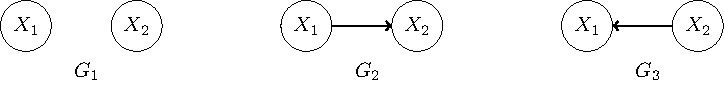
\includegraphics{./picture/bivariate.pdf}
  \caption{2変数のDAGモデル}
  \label{fig:ex_bivariate}
\end{figure}

命題\ref{prop:MRS}より、$G_1$におけるすべての頂点$j \in \{ 1,2 \}$について、
$E(X_j^2) = E(X_j) + E(X_j)^2$である。
$G_2$においては、以下が成り立つ。
\begin{equation*}
  E(X_1^2) = E(X_1) + E(X_1)^2, \quad \text{and} \quad
  E(X_2^2) > E(X_2) + E(X_2)^2
\end{equation*}
同様に、$G_3$においては、以下が成り立つ。
\begin{equation*}
  E(X_1^2) > E(X_1) + E(X_1)^2, \quad \text{and} \quad
  E(X_2^2) = E(X_2) + E(X_2)^2
\end{equation*}
つまり、モーメント比$E(X_j^2) / (E(X_j) + E(X_j)^2)$によって、
真のグラフ構造を同定することが可能である。
